\documentclass[11pt,a4paper]{report}
\usepackage{afterpage}
\usepackage{hyperref}
\hypersetup{
colorlinks,
allcolors=black,
linktoc=all
}
\usepackage{titlesec}
\titleformat{\chapter}[display]{\vspace{-3cm}\normalfont\bfseries}{}{0pt}{\LARGE}
\usepackage[english,main=spanish]{babel}
\usepackage[utf8]{inputenc}
\usepackage{color}
\usepackage[table]{xcolor}
\usepackage{graphicx}
\usepackage[export]{adjustbox}
\usepackage{amssymb}
\usepackage{url}
\usepackage{xcolor}
\usepackage{caption}
\usepackage{float}
\usepackage{listingsutf8}
\usepackage[framemethod=default]{mdframed}
\definecolor{LightGray}{gray}{0.9}
\usepackage{babel}
\usepackage[english]{babelbib}
\definecolor{codegreen}{rgb}{0,0.6,0}
\definecolor{codegray}{rgb}{0.5,0.5,0.5}
\definecolor{codepurple}{rgb}{0.58,0,0.82}
\definecolor{backcolour}{rgb}{0.95,0.95,0.92}
\lstdefinestyle{codigo}{
    backgroundcolor= \color{backcolour},   
    commentstyle=\color{codegreen},
    keywordstyle=\color{magenta},
    numberstyle=\tiny\color{codegray},
    stringstyle=\color{codepurple},
    basicstyle=\scriptsize\normalfont\sffamily,  
    breakatwhitespace=false,         
    breaklines=true,                 
    captionpos=t,                 
    keepspaces=true,
    numbers=left,                   
    numbersep=5pt,  
    showspaces=false,                
    showstringspaces=false,
    showtabs=false,                  
    tabsize=2,
    frame=single,
    framexleftmargin=15pt,
    framexrightmargin=5pt,
    framexbottommargin=5pt,
    framextopmargin=5pt,
    inputencoding=utf8,
    extendedchars=true,
    literate = {¬}{{$\neg$}}1
}

\DeclareCaptionFormat{listing}{#1#2#3}
\captionsetup[lstlisting]{format=listing,singlelinecheck=false, margin=0pt, font={sf},labelsep=space,labelfont=bf}


\renewcommand{\lstlistingname}{Código}
\renewcommand{\lstlistlistingname}{Índice de códigos}

\usepackage[many]{tcolorbox}  
\newtcolorbox{boxB}{
    boxrule = 1.5pt,
    colframe = white,
    rounded corners,
    arc = 5pt
}

\definecolor{mygreen}{rgb}{0,0.6,0}
\definecolor{mygray}{rgb}{0.5,0.5,0.5}
\definecolor{mymauve}{rgb}{0.58,0,0.82}
\definecolor{terminalbgcolor}{HTML}{330033}
\definecolor{terminalrulecolor}{HTML}{000099}

\lstdefinestyle{terminal}
{
    backgroundcolor=\color{black},
	basicstyle=\scriptsize\color{white}\ttfamily,
	breaklines=true,
	captionpos=t,
	extendedchars=true,
	showspaces=false,
	showstringspaces=false,
	frame=single,
    framexleftmargin=5pt,
    framexrightmargin=5pt,
    framexbottommargin=5pt,
    framextopmargin=5pt,
    breakindent=0pt,
    breakautoindent=false,
    literate={\$}{{\$}}1 
         {:}{{:}}1
         {¬}{{$\neg$}}1
         {~}{{\textasciitilde}}1,
}

\begin{document}

\begin{titlepage}
\begin{center}


\includegraphics[height=2.38cm]{imagenes/logo_uc.png}
\vspace{0.4cm}

\textbf{Facultad de Ciencias}

\vspace{1cm}

\LARGE
\textbf{Modelado del caudal natural en la cuenca hidrográfica Chambo con Redes Neuronales}

Título en inglés

\vspace{1.cm}
Trabajo de Fin de Máster


\vspace{0.5cm}
\textbf{Anabela Romina Turlione}

\vspace{0.3cm}
\small
\textbf{Director }: Felipe Fernandez Perez\\
\textbf{co Director }: Manuel de Jesus Peñil




% \Large
% Facultad de Informática\\
% Universidad Nacional de La PLata
\end{center}


% \begin{figure}[t]
%     \raggedright
%       
\includegraphics[scale=1]{Figures/Portada.pdf}
        
%   \end{figure}


\end{titlepage}
\afterpage{\null\thispagestyle{empty}\newpage}
\chapter*{Agradecimientos}
\markboth{AGRADECIMIENTOS}{AGRADECIMIENTOS}
\thispagestyle{empty}
Página de agradecimientos

\tableofcontents
\thispagestyle{empty}

\lstlistoflistings
\thispagestyle{empty}

\listoffigures
\thispagestyle{empty}

\setcounter{page}{1}
\chapter*{Resumen}
\addcontentsline{toc}{chapter}{Resumen}

En este trabajo se ha evaluado el desempeño de diferentes modelos de redes neuronales
para predecir el caudal natural en la cuenca hidrográfica Chambo  a partir de series de
entrada hidro-climáticas que abarcan un rango de 14 años. Se han considerados redes con
diferentes estructuras y se han entrenado de manera local, global y secuencial. Se ha medido el
desempeño de los modelos utilizando diferentes métricas y se ha comprobado que en la
mayoría de los casos, los modelos logran reconstruir de manera correcta los caudales en un
rango de 6 años. Con los resultados obtenidos se ha utilizado el software de gestión Modsim
que permite optimizar los usos de los recursos de la cuenca y se ha comprobado que los
resultados obtenidos por medio de los modelos de redes neuronales son los mismos que los obtenidos con un
modelo hidrológico tradicional. Finalmente se ha desarrollado una aplicación que permite la ejecución del modelo
en diferente cuencas hidrológicas.\\
\\
\textbf{Palabras claves:} Redes Neuronales, redes recurrentes, hidrología, predicción, cuencas hidrográficas, aprendizaje automático, aprendizaje profundo\\
\\
\\
\large{\textbf{Abstract}}
\vspace{5mm}

In this work, the performance of different neural network models
to predict the natural flow in the  watershed Chambo  has been evaluated. 
Models with different configurations  have been trained locally, globally and sequentially  in 
hydro-climatic series spanning a 14-year range.
The performance of the models, has been measured
using different metrics, and it has been verified that in most cases, they succeed in correctly reconstructing the flows over a
6 year range. The obtained results  has been used to optimize the use of the resources of the basin with the software Modsim, 
and it has been proven that the the results obtained by means of neural network models are the same as those obtained with a
traditional hydrological model. Finally, an application has been developed that allows the execution of the model
in different hydrological basins.\\
\\
\textbf{Key words:} Neural Networks, recurrent networks, hydrology, prediction, hydrographic basin, machine learning, deep learning
\chapter{Introducción}
\label{introduccion}

Introducción de la tesis

Ejemplo de secciones

\section{Motivación}

Motivación de la tesis.

Un ejemplo de cita.\cite{web:unlp}

\section{Objetivos y metodología}

Objetivos y metodología.

\section{Resultados obtenidos}

Resultados obtenidos

\section{Organización del documento}

Organización del documento

\begin{itemize}
    \item Capítulo 1.
    \item Capítulo 2.
    \item Capítulo 3.
\end{itemize}
\chapter{Cuenca del río Chambo}
\label{capitulo 1}
\section{Descripción del sistema}
% \section{Red fluvial}
% \section{Usos de agua}
% \section{Aportaciones}
\chapter{Descripción y exploración de los datos}
\label{capitulo 1}


En este capítulo se describen las características principales de las series temporales hidroclimáticas utilizadas 
tanto para entrenar los modelos de aprendizaje profundo como para generar las variables objetivos, es describe
los caudales de descarga de las subcuencas con el modelo hidrológico LEM.



\section{Series de precipitación}


La cuenca del río Chambo posee una gran variación en la precipitación en un área geográfica reducida,
por este motivo los valores de precipitación recogidos por pluviómetros en las estaciones meteorológicas 
pueden no son fácilmente extrapolables a puntos más lejanos. Por otro lado los pluviómetros se encuentran 
a altitudes de entre los 2000 y 3000 metros sobre el nivel del mar, mientras que el punto más alto de la cuenca se encuentra a las 6288 m.s.n.m,
Lo que da lugar a que haya una deficiencia de datos en ciertos puntos geográficos de la cuenca. Para completar los datos en Estos
puntos se ha recurrido a las base de datos de ERA5 \cite{ERA5} y CHELSA \cite{CHELSA}.


Con el fin de contrastar si estas series reflejan 
correctamente las variaciones del patrón de lluvias con la altura y la pendiente, 
se han analizado diversas bases de datos globales de precipitación pero el resultado no ha sido 
satisfactorio.  Por ello, se ha optado por generar las series de precipitación de manera sintéticas basándose 
en los patrones combinados de los pluviómetros y de las estaciones de aforos.



% Los datos de clima (precipitación y temperatura) fueron medidos a través de estaciones meteorológicas distribuidas de manera 
% irregular a lo largo de la cuenca. Las series disponibles reflejan adecuadamente las condiciones climáticas de las zonas 
% bajas y más pobladas, pero la información en las zonas más altas es escasa. 
% Los pluviómetros se encuentran a altitudes de entre los 2000 y 3000 metros sobre el nivel del mar, 
% mientras que el punto más alto de la cuenca se encuentra a las 6288 m.s.n.m

% Con el fin de contrastar si estas series reflejan 
% correctamente las variaciones del patrón de lluvias con la altura y la pendiente, 
% se han analizado diversas bases de datos globales de precipitación pero el resultado no ha sido 
% satisfactorio.  Por ello, se ha optado por generar las series de precipitación de manera sintéticas basándose 
% en los patrones combinados de los pluviómetros y de las estaciones de aforos.

% La cuenca del río Chambo posee una gran variación en la precipitación en un área geográfica reducida,
% por este motivo los valores de precipitación recogidos por pluviómetros en las estaciones meteorológicas 
% pueden no ser válidos para puntos lejanos. Es por eso que los datos correspondientes a puntos intermedios se 
% completaron a partir de la base de datos de ERA5 y CHELSA.

% \begin{figure}[h!]
%   \begin{center}
%     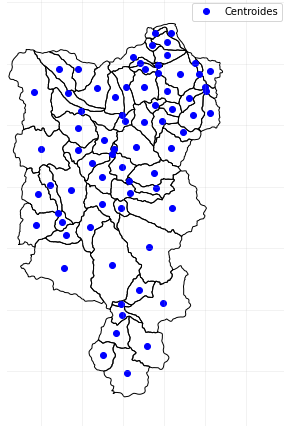
\includegraphics[height=3.in]{Figures/centroides.png}
%     \caption{ Localización de los centroides de las subcuencas}
%     \label{0}
%   \end{center}
% \end{figure}

%  Una vez que los huecos han sido rellenados, se han interpolado los datos recogidos por los pluviómetros a los centroides 
%  de las regiones  representadas en la figura \ref{0}. Este proceso consta de dos pasos, primero se estima si en un punto 
%  determinado va a llover (estimación kriging con la librería \textit{Krige} de r) y luego se estima la magnitud de dicha 
%  lluvia (Herrera et al., 2012).

%  \begin{figure}[h!]
%   \begin{center}
%     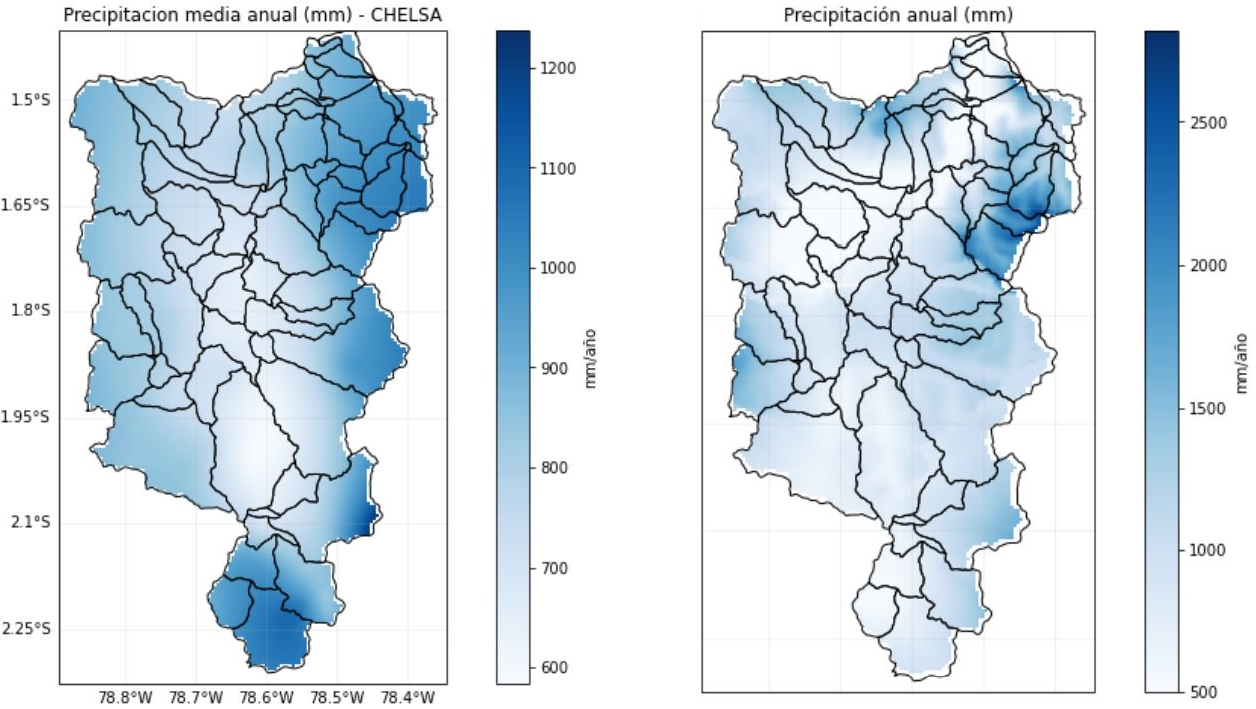
\includegraphics[height=3.in]{Figures/CHELSA_ERA5.jpg}
%     \caption{ Precipitación media anual (mm/año) basada en CHELSA (panel izquierdo) y en ERA5 (panel derecho).}
%     \label{1}
%   \end{center}
% \end{figure}


%  En la figura \ref{1} se muestra a modo de ejemplo los  valores de la precipitación media anual  obtenidos mediante interpolación 
%  sobre una malla regular de 100 m de lado utilizando la base de datos de ERA5 (panel derecho) y la de CHELSA (panel izquierdo).
%  Si bien los resultados reflejan correctamente la fuerte variabilidad de la precipitación en un area reducida, los patrones estacionales
%  así obtenidos no coinciden con los caudales y el conocimiento local. Es por eso que se ha optado por generar las series 
%  de manera sintética como se describe en la siguiente sección.



El modelo que genera las series de precipitación diaria consta de dos niveles, primero se generan series mensuales y
luego se generan series diarias desagregando los valores mensuales.
Para generar las series mensuales se parte del valor medio anual en la región de interés y del valor medio en el 
mes más húmero
% . Se han definido a su vez, tres patrones de precipitación para diferentes regiones:
% 1) costero, donde la precipitación máxima tiene lugar en el mes de abril, y un segundo pico inferior al de abril, en torno a octubre-noviembre.
% 2) amazónico, con un único pico de precipitación en junio-julio, y el mínimo en diciembre-enero y 3) mixto que es una combinación de los dos primeros. 

La precipitación media anual  se determina mediante en la interpolación de los datos de los
pluviómetros con la base de datos CHELSA ya que en términos de magnitud es la más exacta.
El modelo de desagregación a escala mensual asume que las precipitaciones acumuladas en cada mes siguen un comportamiento
que puede ser representado por la siguiente distribución "Log-normal" que posee una variación temporal sinusoidal y
desviación estándar $s_1$:

\begin{equation}
    P_m=exp\Bigg(N\bigg(a+b1\cdot cos\bigg(\frac{t-\phi_1}{6}\bigg)+b2\cdot cos\bigg(\frac{t-\phi_2}{12}\bigg)\bigg)\Bigg)
\end{equation}

$N(\mu,\sigma)$ es a su vez una distribución Gaussiana con media $\mu$ y desviación estándar $\sigma$. 
Los valores de las constantes $a$, $b_1$ y $b_2$ se obtienen a partir de la precipitación media y máxima, 
mientras que las fases $\phi_i$ dependen del régimen de precipitación.

% \begin{figure}[h!]
%     \begin{center}
%       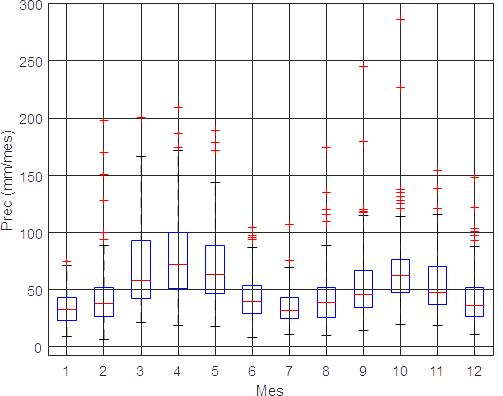
\includegraphics[height=3.in]{Figures/prec_sim.png}
%       \caption{ Valores simulados de precipitaciones mensuales en la zona de Guaslán}
%       \label{2}
%     \end{center}
%   \end{figure}


% En la figura \ref{2} se muestra a modo de ejemplo una de las series generada para una cuenca con clima costero, representativa del sector más 
% seco de la cuenca en la estación de Guaslán (cantón Riobamba). La línea roja representa el valor medio, la caja azul representa los valores situados entre los percentiles
%  25$\%$ y 75$\%$, y las barras negras los extremos (los puntos en rojo son tratados como datos atípicos). A modo de comparación,
%  en la figura \ref{3} se muestran los valores observados en la misma estación.

%  \begin{figure}[h!]
%     \begin{center}
%       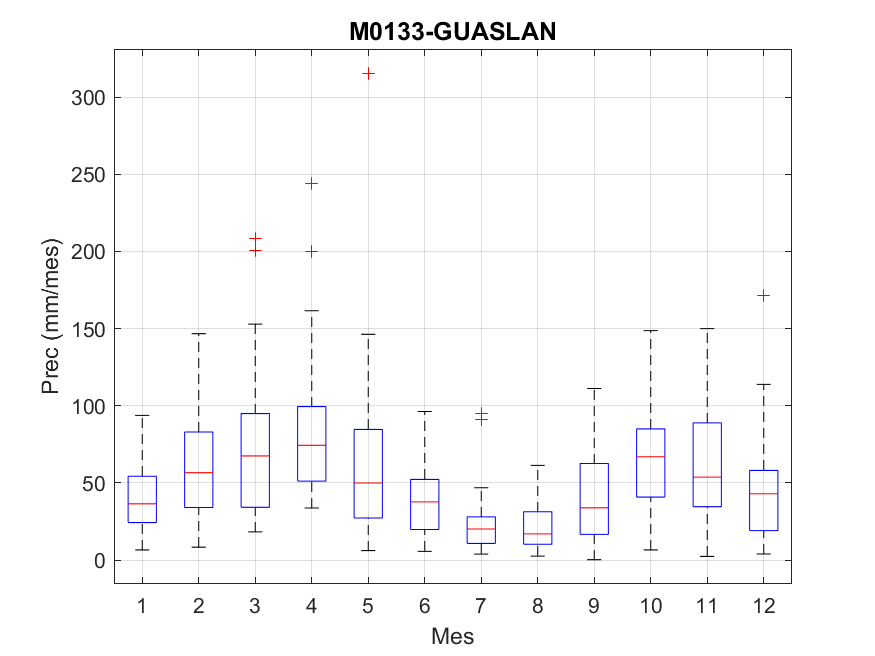
\includegraphics[height=3.in]{Figures/prec_obs.png}
%       \caption{ Valores observados de precipitaciones mensuales en la zona de Guaslán}
%       \label{3}
%     \end{center}
%   \end{figure}

%   \begin{figure}[h!]
%     \begin{center}
%       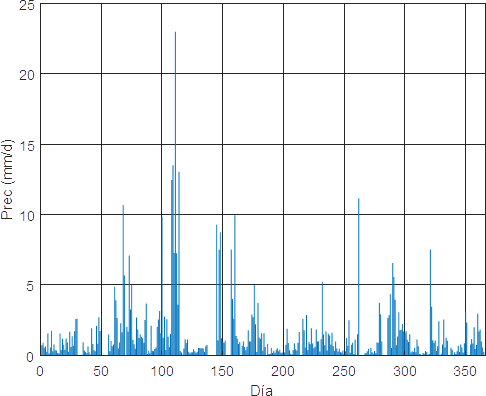
\includegraphics[height=3.in]{Figures/prec_sint.png}
%       \caption{ Un año de valores de precipitación diaria simulada en la zona de Guaslán}
%       \label{3}
%     \end{center}
%   \end{figure}


El modelo para crear las series diarias usa el método de cascadas aleatorias multiplicativas \cite{Molnar} para 
desagregar las series mensuales. El modelo consta de dos parámetros: denominados $sig2$ y $beta$
que determinan la variabilidad e intermitencia de la lluvia (proporción media de días sin lluvia) y se usan para 
ajustar el modelo, con los valores observados en las series de precipitación disponibles.


% \subsubsection{Comportamiento del régimen de precipitación}
% \label{regimenes_prec}
% Con el fin de poder realizar un estudio completo de cómo es el comportamiento del régimen de precipitaciones, 
% se seleccionaron 35 estaciones  meteorológicas que abarcan de manera uniforme el area de la cuenca de Chambo y sus alrededores.
% Se han identificado principalmente dos regímenes diferentes, un régimen bimodal en el oeste (dos períodos secos y dos de lluvias al año) 
% y el régimen monomodal (un período seco y uno de lluvias) en el este, con una franja que contiene un régimen mixto en 
% las zonas centrales de la cuenca.










\section{Series de temperatura}
\label{tempint}
Para la generación de las series de temperatura se utilizado datos de 10 termómetros situados en el entorno del área de estudio.
Estos datos han sido sometidos al un proceso de curado que por un lado define una frontera para detectar outliers o datos atípicos
siguiendo el siguiente criterio:
\begin{equation}
  si~X_i>5\cdot\sigma^2_n~es~un~utlier,~donde~\sigma^2_n=\frac{1}{n}\cdot\sum^n_{i=1}\bigg(X_i-\bar{X}\bigg)^2
\end{equation}
y por el otro lado elimina los datos que presentan un cierto grado de persistencia \cite{Estevez}
Los datos faltantes se han completados de manera similar a cómo se procedió con las series 
de precipitación utilizando los datos de ERA5.


\begin{figure}[h!]
  \begin{center}
    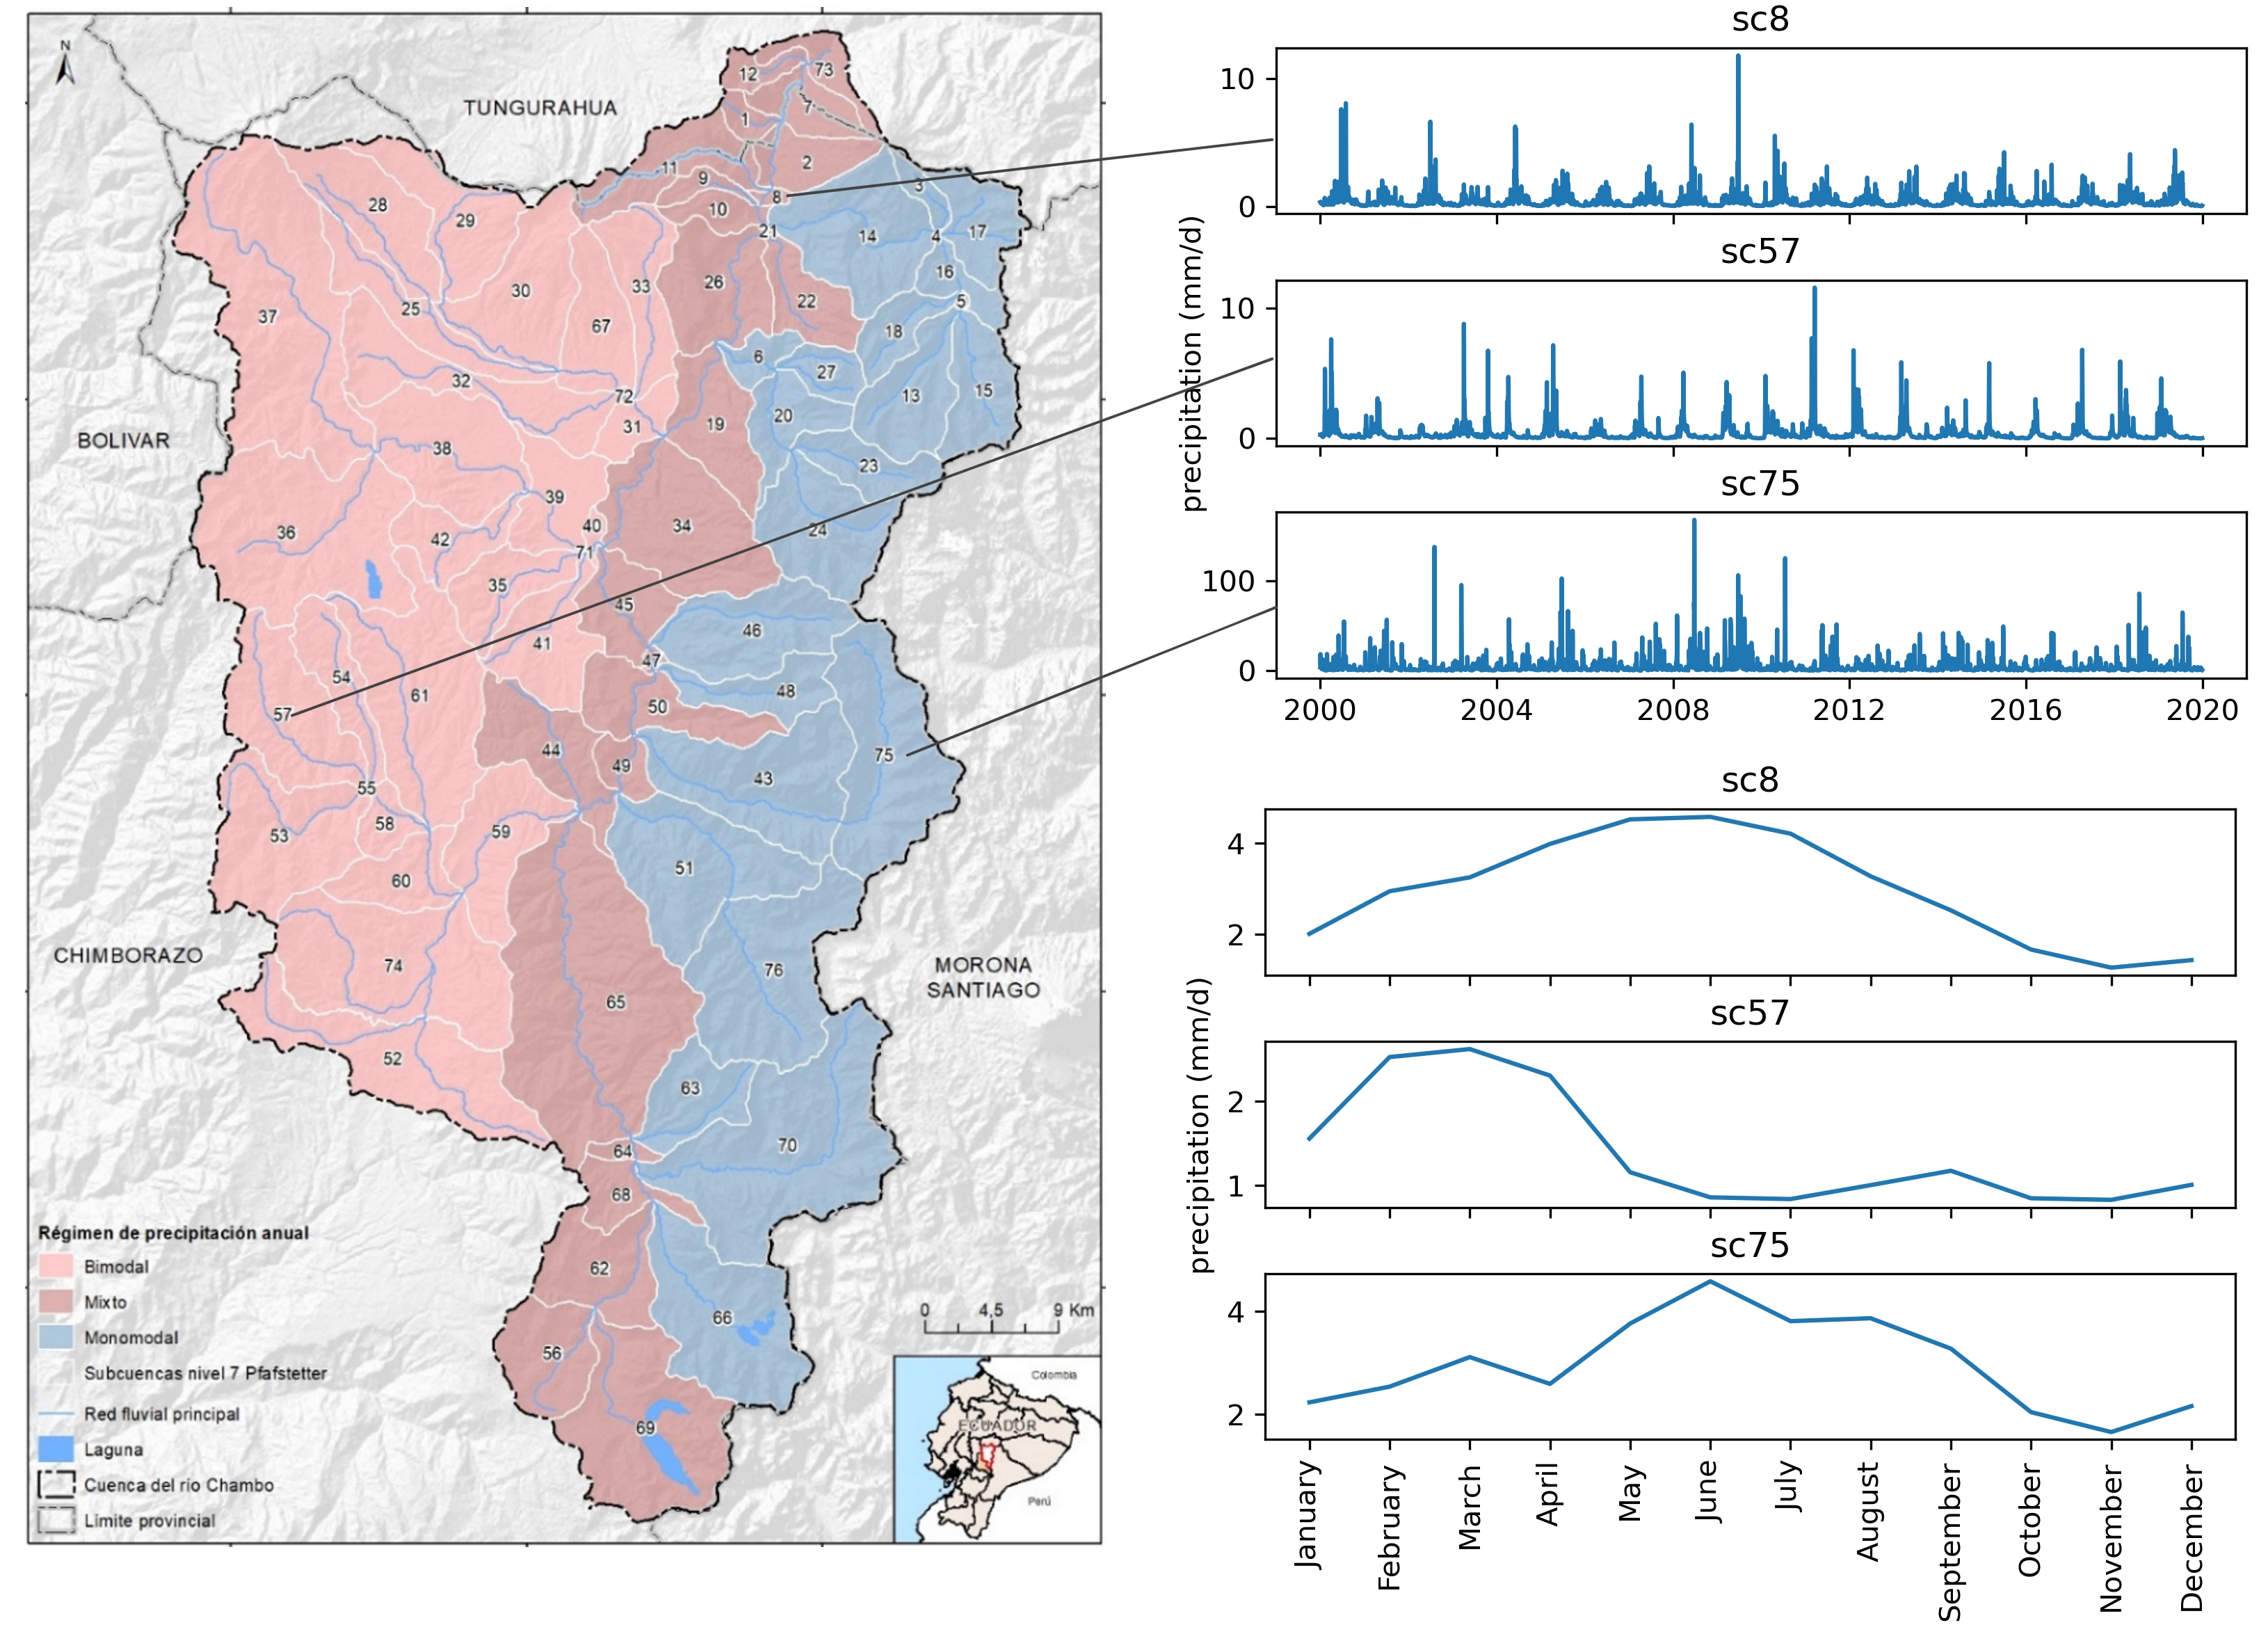
\includegraphics[height=6.5in]{Figures/cuenca_con_subcuencas_prec.png}
    \caption{ Series de precipitación para diferentes regiones de la cuenca Chambo. En los panel superior derechos se muestra la serie 
    de precipitación correspondiente al año 2019 y  los valores medios mensuales desde el año 2000 hasta el año 2020. En el panel 
    inferior, se muestran las series de temperatura máxima y mínima diarias.}
    \label{4}
  \end{center}
\end{figure}

En la figure \ref{4}, se muestran a modo de ejemplo las series de precipitación y temperaturas
mínimas y máximas generadas para tres diferentes subcuencas 
localizadas en diferentes puntos. Se puede observar las diferentes estacionalidades,
la cuenca con id = 57 presenta un  un régimen costero (donde la precipitación máxima tiene lugar en el mes de abril), 
las cuencas con ids= 8 y 75, un régimen amazónico (con un único pico de precipitación en junio-julio).



\chapter{Modelo Hidrológico}
\label{Modelo_Hidrológico}

Cómo se ha descrito anteriormente, se ha utilizado el modelo hidrológico MELCA
 para generar las series de caudales de descarga que han sido utilizadas como variables objetivos
al entrenar los modelos de redes neuronales (capítulo \ref{ANNs}). 
 Este modelo está basado en LEM y fue desarrollado por IHCantabria.
 A continuación se describen las características principales de estos modelos.

\section{Modelo LEM}

Este modelo simula el proceso hidrológico en una cuenca hidrográfica a partir de las siguientes hipótesis empíricas:
\begin{enumerate}
    \item Las cuencas hidrográficas son sistemas complejos que persiguen continuamente un equilibrio dinámico, 
    dado por una combinación de factores climáticos ( precipitación y evapotranspiración potencial) 
    y algunas características del terreno (topografía, vegetación, suelo, geología, etc.). 

    La evolución de la escorrentía ($R$) hacia el equilibrio sigue la ley clásica de crecimiento descrito por la 
    ecuación logística:

    \begin{equation}
        \frac{d R(t)}{dt}=K\cdot R(t)\cdot\big(1-\frac{R(t)}{R_{eq}}\big)
    \label{eq.log}
    \end{equation}

    \item  $Req$ es la escorrentía de equilibrio  y se puede expresar como un coeficiente de escorrentía de 
    equilibrio ($Ceq$) multiplicado por la precipitación instantánea: $Req = P \cdot Ceq$. 
    
    \item $K$ es la tasa de crecimiento y es una función lineal de la precipitación: $K=P/S_0$ , donde $S_0$ 
    es una constante con unidades de longitud ($mm$) que representa un espesor característico del suelo.
    \item La ecuación logística no considera el  tiempo de viaje desde las 
    zonas de producción de escorrentía hasta el punto final de medida del caudal, en la salida de la cuenca. 
    Cuando el intervalo de tiempo de análisis es del mismo orden de magnitud que el tiempo 
    de respuesta de una cuenca, se debe agregar un método de propagación.


\end{enumerate}

La versión estándar del LEM adopta un modelo lineal para el submodelo de enrutamiento y toma la forma del siguiente sistema 
de ecuaciones:


\begin{equation}
    \frac{d R(t)}{dt}=\frac{P(t)}{S_0}\cdot R(t)\cdot\big(1-\frac{R(t)}{R_{eq}}\big)
\end{equation}

\begin{equation}
    \frac{d \hat{P}}{dt}=P(t)-\frac{\hat{P}}{\lambda}
\end{equation}


\begin{equation}
    \frac{d \hat{E}}{dt}=E(t)-\frac{\hat{E}}{\lambda}
\end{equation}


\begin{equation}
    R_{eq}(t)=P(t)\cdot C_{eq}(\psi);\ \ C_{eq}(\psi)=e^{-a\cdot \psi}, \psi=\frac{\hat{E}}{\hat{P}}
\end{equation}


\begin{equation}
    \frac{d Q(t)}{dt}=\frac{1}{\tau}\cdot \big[R(t)-Q(t)\big]
\end{equation}


Donde $R$ y $Q$ son la escorrentía total y la descarga medida en la salida de la cuenca, respectivamente. 
$P$ y $E$ son la precipitación y la evapotranspiración potencial en cada paso de tiempo, mientras que $\hat{P}$ y $\hat{E}$ 
son valores promediados de $P$ y $E$ durante un periodo de tiempo característico, respectivamente. 
Los parámetros del modelo entonces son:
\begin{itemize}
    \item $\lambda$ (días), el tiempo característico de respuesta  de la cuenca. %($1/(25.465*log(s0)-19.494)$).
    \item $S_0$ (mm), que representa un espesor medio de suelo o una capacidad de almacenamiento característica de la cuenca.
    \item $a$, un parámetro adimensional que modifica la forma de la función de equilibrio (típicamente en el rango 0.5-1.5)
    \item $\tau$ (horas), el parámetro de enrutamiento, que puede considerarse un tiempo 
    de respuesta rápido de la cuenca.
\end{itemize}
Este sistema de ecuaciones diferenciales ordinarias puede resolverse numéricamente con un esquema explícito 
incondicionalmente estable, ya que  que todas las ecuaciones, y en especial la logística, tienen solución analítica.

Como se ha mencionado en el capítulo \ref{datos}, los datos de precipitación correspondientes a las zonas más 
altas de la cuenca son escasos. Es por esto que es necesario aplicar  dos factores $fcp$ y $fce$ 
que tienen en cuenta la influencia de la altitud de cada subcuenca y
 sirven para calibrar el modelo y corregir las series de precipitaciones y evo-transpiración, respectivamente.
 Para calibrar el modelo se han utilizado datos de caudales recogidos por diferentes estaciones de aforo proporcionados por
 MAATE \cite{MAATE} y los valores de caudal promedio aportados por el documento de ``\textit{Aportes a la planificación para 
 la gestión integral de los recursos hídricos}'' citado en \cite{Rodriguez}. 
 El modelo es entonces calibrado en cada sub-cuenca de manera individual, ajustando los factores de corrección $fcp$ y $fce$ 
 de modo tal que los caudales   mensuales medios  simulados se acerquen lo más posible a los valores medidos en las estaciones de aforo.
 
 
%  \begin{figure}[h!]
%      \begin{center}
%        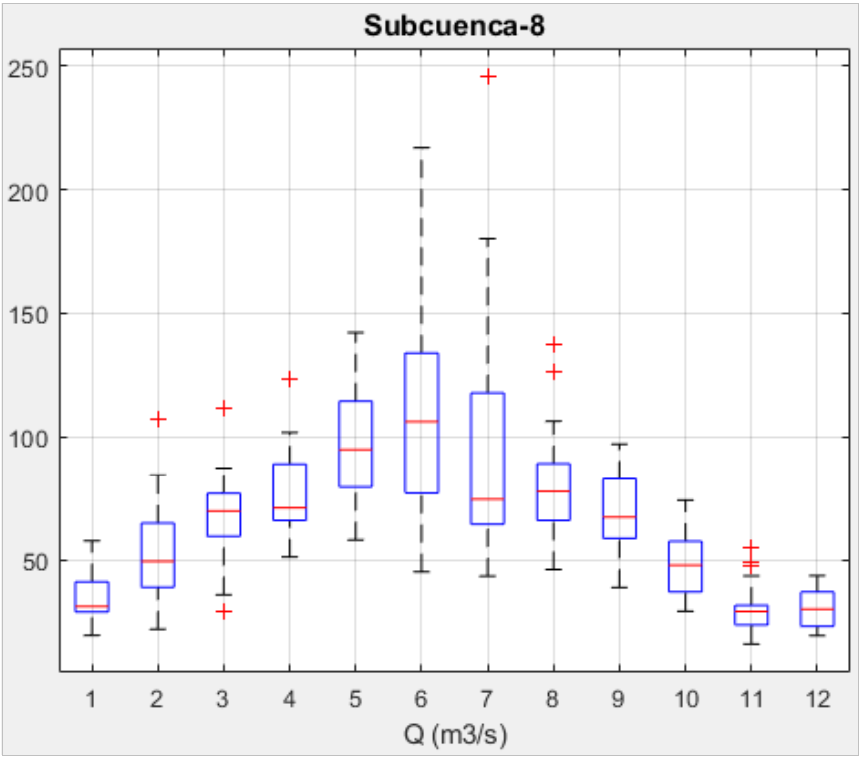
\includegraphics[height=3.in]{Figures/caudal_sim.PNG}
%        \caption{ Valores simulados de caudales mensuales para la subcuenca 8.}
%        \label{2}
%      \end{center}
%    \end{figure}
 
 
 
%   \begin{figure}[h!]
%      \begin{center}
%        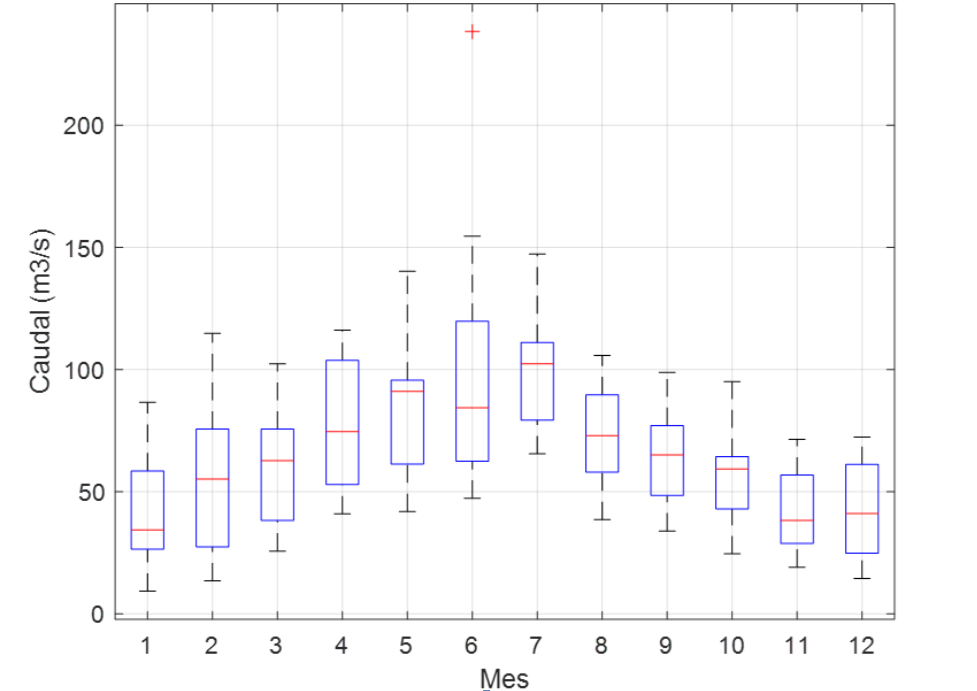
\includegraphics[height=3.in]{Figures/caudal_obs.PNG}
%        \caption{ Valores observados de caudales mensuales para la subcuenca 8.}
%        \label{3}
%      \end{center}
%    \end{figure}
 
 
 
%    En la figura \ref{2} se muestran a modo de ejemplo, los valores observados (panel inferior) y simulados  (panel superior) para la subcuenca 8.
%    La línea roja representa el valor medio, la caja azul representa los valores situados entre los percentiles
%    25$\%$ y 75$\%$, y las barras negras los extremos (los puntos en rojo son tratados como datos atípicos). 
%     Se puede observar que a calibración ha ayudado a igualar considerablemente los caudales modelados con los caudales aforados.



\subsection{Modelo MELCA}

MELCA es un modelo hidrológico semi-distribuido basado en LEM. 
Este modelo considera varias subcuencas, cada una de ellas con sus parámetros y forzamientos climáticos diferenciados
y permite incluir una serie de particularidades asociadas a las cuencas tropicales andinas como la inclusión de páramos 
y bofedales con sus topologías y el estado de conservación. El modelo convierte la superficie de cada uno de estos 
ecosistemas andinos en una capacidad equivalente de almacenamiento del suelo. 
También  incluye factores de corrección para  la evo-transpiración en zonas de alta montaña, el efecto de glaciares 
y la aportación de agua atmosférica proveniente de niebla (flujo que es significativo en zonas cuencas andinas tropicales). 


\begin{figure}[h!]
    \begin{center}
      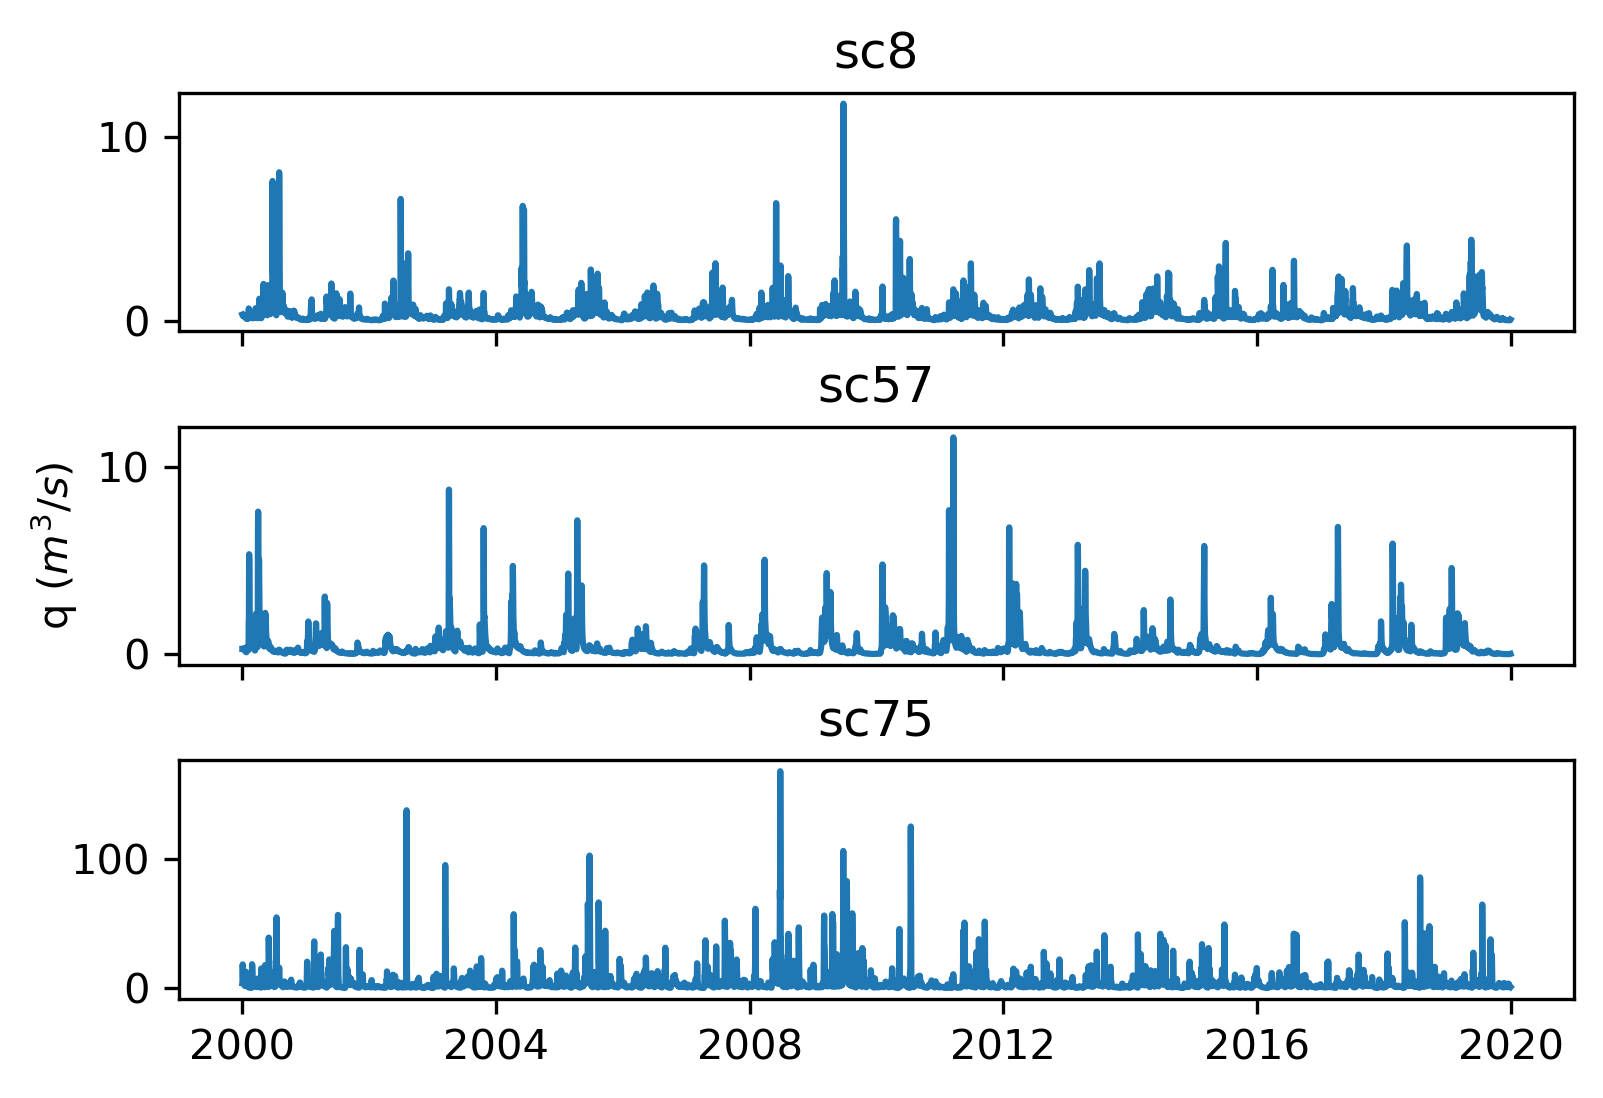
\includegraphics[height=3.5in]{Figures/caudales.png}
      \caption{ Caudales diarios simulados con el modelo MELCA para las cuencas con ids 8, 57 y 75 desde el año 2000 hasta
      el año 2020. }
      \label{caudales}
    \end{center}
  \end{figure}

En la figura \ref{caudales} se muestran a modo de ejemplo los caudales de descarga diarios simulados con el modelo MELCA 
para las cuencas con ids 8, 57 y 75. Se puede observar que la cuenca 75, que se encuentra más cerca del amazonas y con 
un régimen más húmedo, posee una caudal considerablemente mayor.
% \subsection{Parámetros físicos}
% El modelo LEM  usa 5 parámetros de entrada, el área de la cuenca, 
% el almacenamiento característico $s_0$, el parámetro de enrutamiento $\tau$, 
% el factor corrector de las precipitaciones $fcp$ y el factor corrector de la evo-transpiración $fce$. 

% \subsubsection{Capacidad de almacenamiento}
% La capacidad de almacenamiento del terreno se ha estimado mediante el método del Número de 
% Curva del \textit{Soil Conservation Service} (SCS).

% Si consideramos que para una cantidad de precipitación $P$, una cantidad $P_e$ se escurre directamente y una cantidad
% $I_a$ se infiltra inicialmente. Por otro lado, una cantidad de agua $F_a$ es retenida y es  
% menor a la capacidad máxima de almacenamiento de la cuenca $S_{max}$.

% El método SCS supone que entre todas las cantidades descriptas, se satisface la siguiente relación:
% \begin{equation}
%     \frac{F_a}{S_{max}}=\frac{P_e}{P-I_a}
% \end{equation}

% Si además aplicamos el principio de continuidad para la precipitación, $P = P_e+I_a+F_a$ y la relación experimental
% entre $S_{max}$ y $I_a$, $I_a=0,2\cdot S_max$, obtenemos una relación entre $P_e$ y $S_{max}$:

% \begin{equation}
%     P_e=\frac{(P-0,2\cdot S_{max})^2}{P-0,8\cdot S_{max}}
% \end{equation}


% El número de curva (CN) se relaciona con la capacidad de almacenamiento máxima de la cuenca de la siguiente manera:

% \begin{equation}
%     S_{max}=25,4\cdot\bigg(\frac{1000}{CN}-10\bigg)
% \end{equation}

% Los números de curva se encuentran tabulados en función del tipo y uso del suelo (referencia).

% Una vez conocidas las capacidades máximas de almacenamiento del suelo por subcuencas, podemos calcular el 
% almacenamiento característico $S_0$, tal y como lo requiere el modelo LEM, antes descrito. 
% De acuerdo a la experiencia de aplicación del modelo en otras cuencas, podemos asumir con  con buen grado de 
% ajuste la siguiente relación:

% \begin{equation}
%     S_{max}=9\cdot S0
% \end{equation}

% \subsubsection{Coeficiente de enrutamiento}

% El parámetro de enrutamiento $\tau$ representa el retardo entre la generación 
% de la escorrentía en el territorio y su llegada al punto de medida en el final de cada tramo. Este parámetro 
% tiene muy poca influencia en el cálculo de los recursos hídricos, ya que no altera el balance de masa, sino que 
% retrasa ligeramente la llegada del caudal (unas horas, mientras que el paso de tiempo de cálculo es un día). 

% \subsubsection{Factores correctores de las precipitaciones}
% Como se ha mencionado en el capítulo \ref{capitulo 1}, los datos de precipitación correspondientes a las zonas más 
% altas de la cuenca son escasos. Es por esto que es necesario aplicar un factor de corrección, $fcp$, a las series de precipitación
% que tiene en cuenta la influencia de la altitud de cada subcuenca, en general las subcuencas que se encuentran a mayor
% altitud tendrán un factor de corrección mayor. 

% \subsubsection{Cálculo de la evapotranspiración corregida}

% La evapotranspiración potencial (ETP) se ha calculado con base en la fórmula de la FAO 56 PM (referencia), 
% que toma los datos de temperatura máxima y mínima de rásteres en cada subcuenca:

% \begin{equation}
%     ETP_0\bigg(\frac{mm}{d}\bigg)=\frac{12,64}{365,25}\cdot \bigg(T_{med}+17,8\bigg)\cdot\bigg(T_{max}-T_{min}\bigg)^{0,5}
% \end{equation}

% Para calcular las temperaturas máximas y mínimas diarias, Tmax y Tmin, se han usado las interpolaciones de los datos 
% instrumentales y la base de datos de ERA5 \ref{tempint}.


% En las cuencas ecuatorianas andinas, la fórmula anterior tiende a sobreestimar la ETP en hasta un 30 $\%$ (Córdova,2015),
% ya que no considera el efecto del aumento de radiación solar ni las condiciones locales de humedad relativa y por otro lado 
% la presencia de viento en esas zonas también distorsiona el valor de ETP. Por lo tanto, se ha aplicado un factor corrector al 
% resultado de la fórmula de la FAO que depende de la altitud y orientación de cada cuenca:

% \begin{equation}
%     ETP\bigg(\frac{mm}{d}\bigg)=f_{ce}\cdot ETP_0\bigg(\frac{mm}{d}\bigg)
% \end{equation}

% \subsubsection{Calibración del modelo}



% \subsubsection{Resultados obtenidos con MELCA}



  

% \begin{figure}[h!]
%     \begin{center}
%       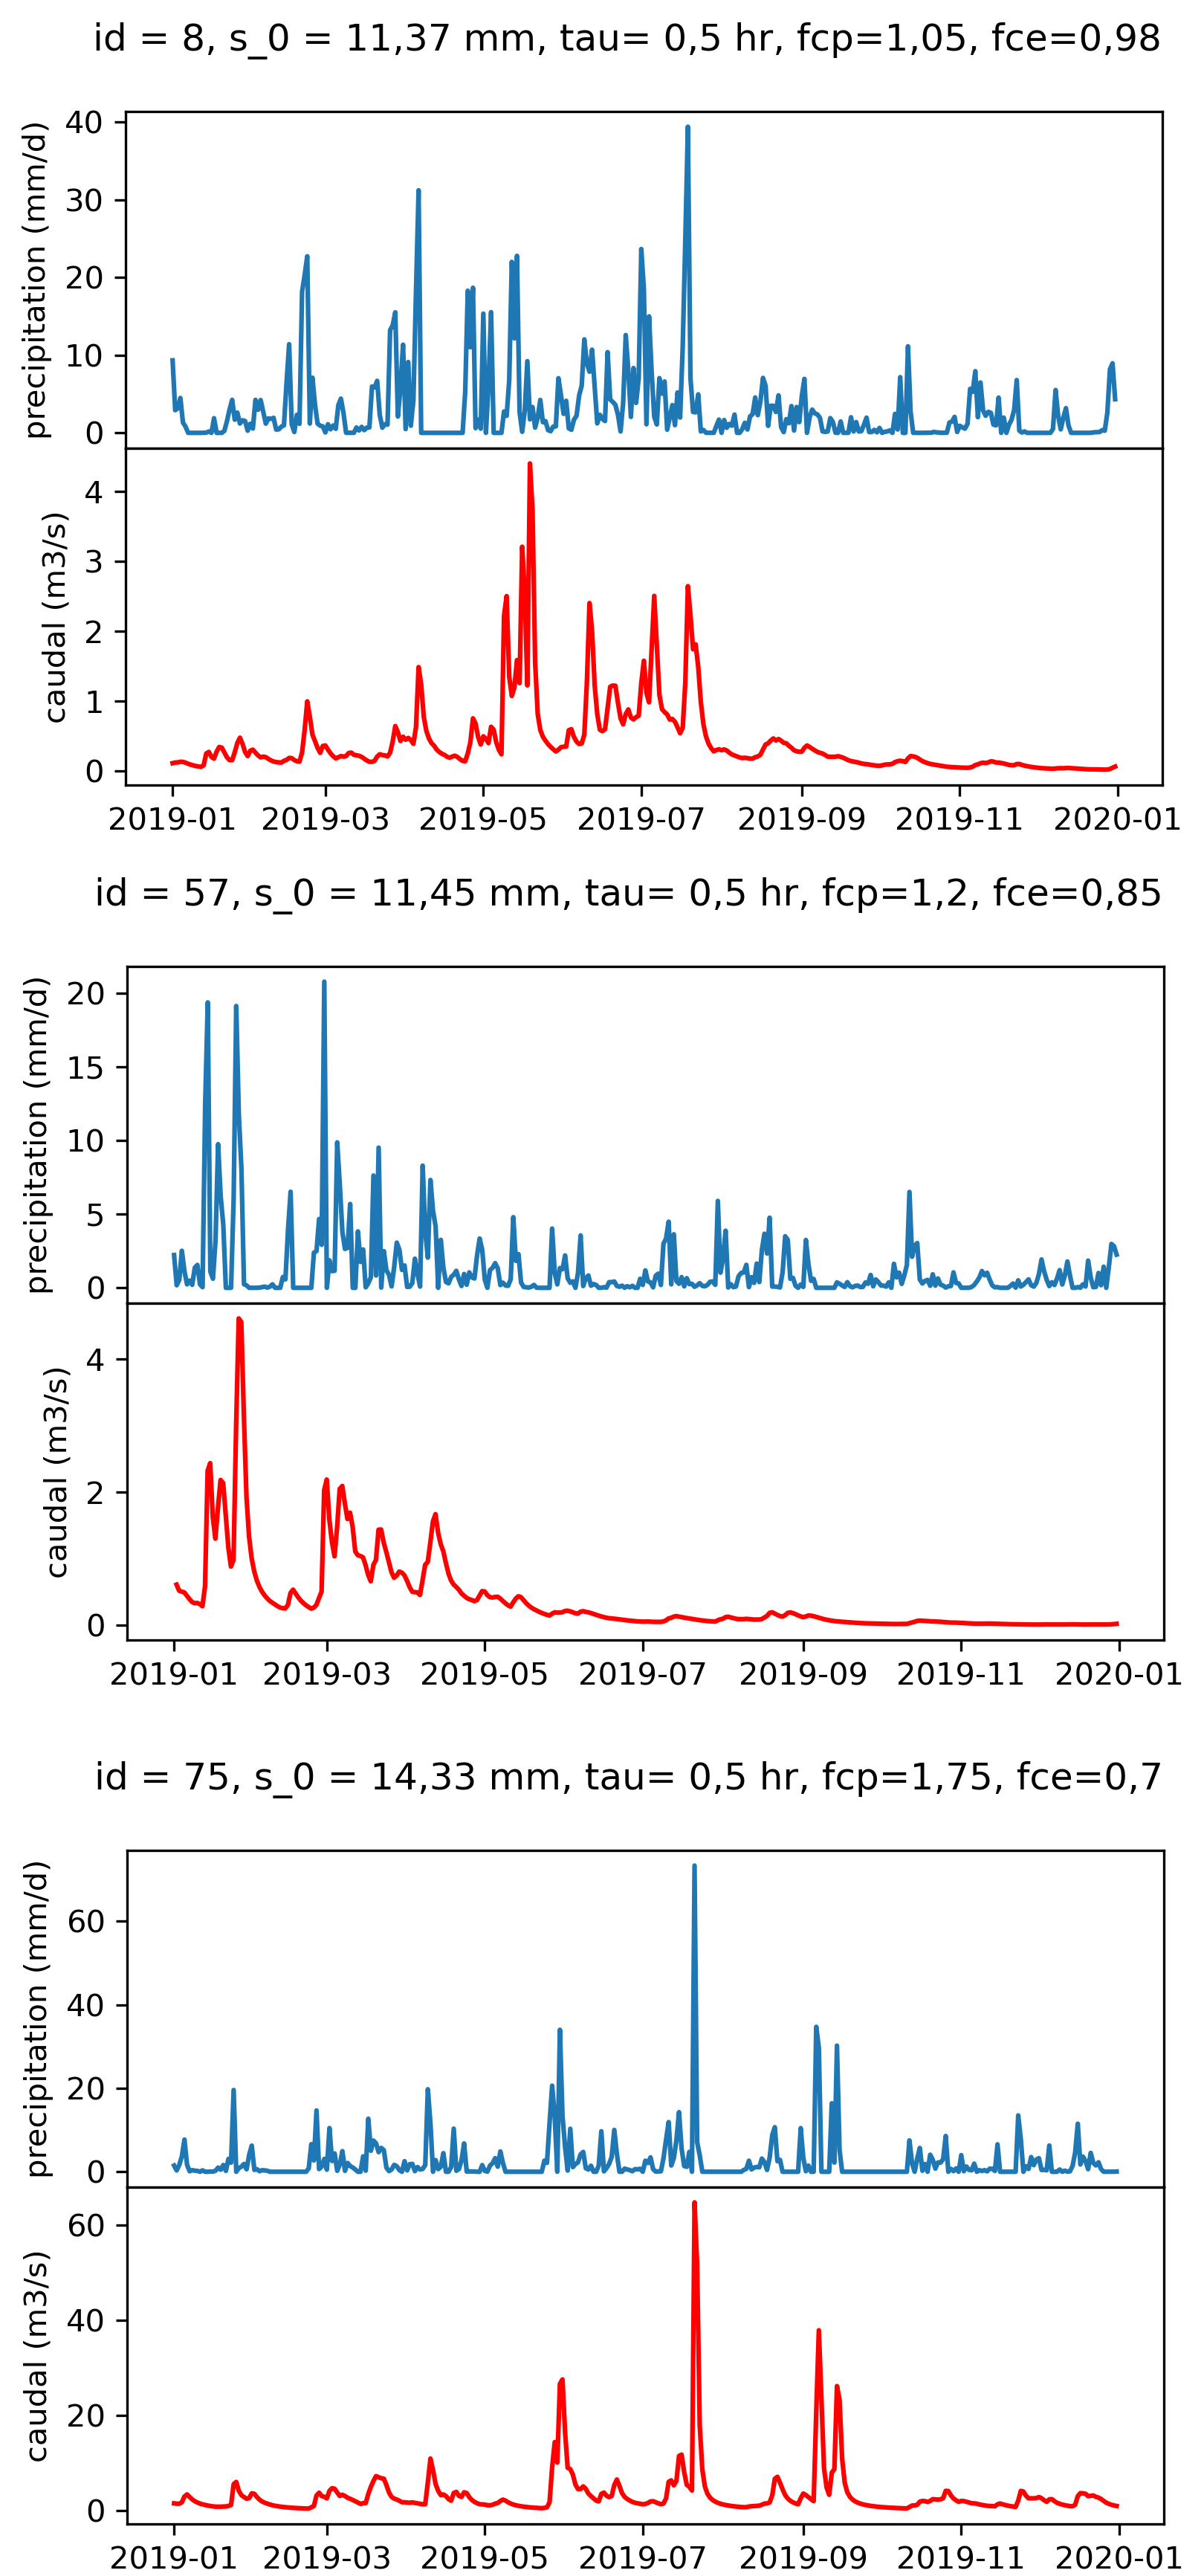
\includegraphics[height=6.5in]{Figures/outputs_MELCA.png}
%       \caption{ Simulaciones de caudales naturales para tres subcuencas durante el añ0 2019, 
%       en las graficas superiores se muestran las series de 
%       precipitación de entrada y los parámetros del modelo.}
%       \label{5}
%     \end{center}
%   \end{figure}

%   \begin{figure}[h!]
%     \begin{center}
%       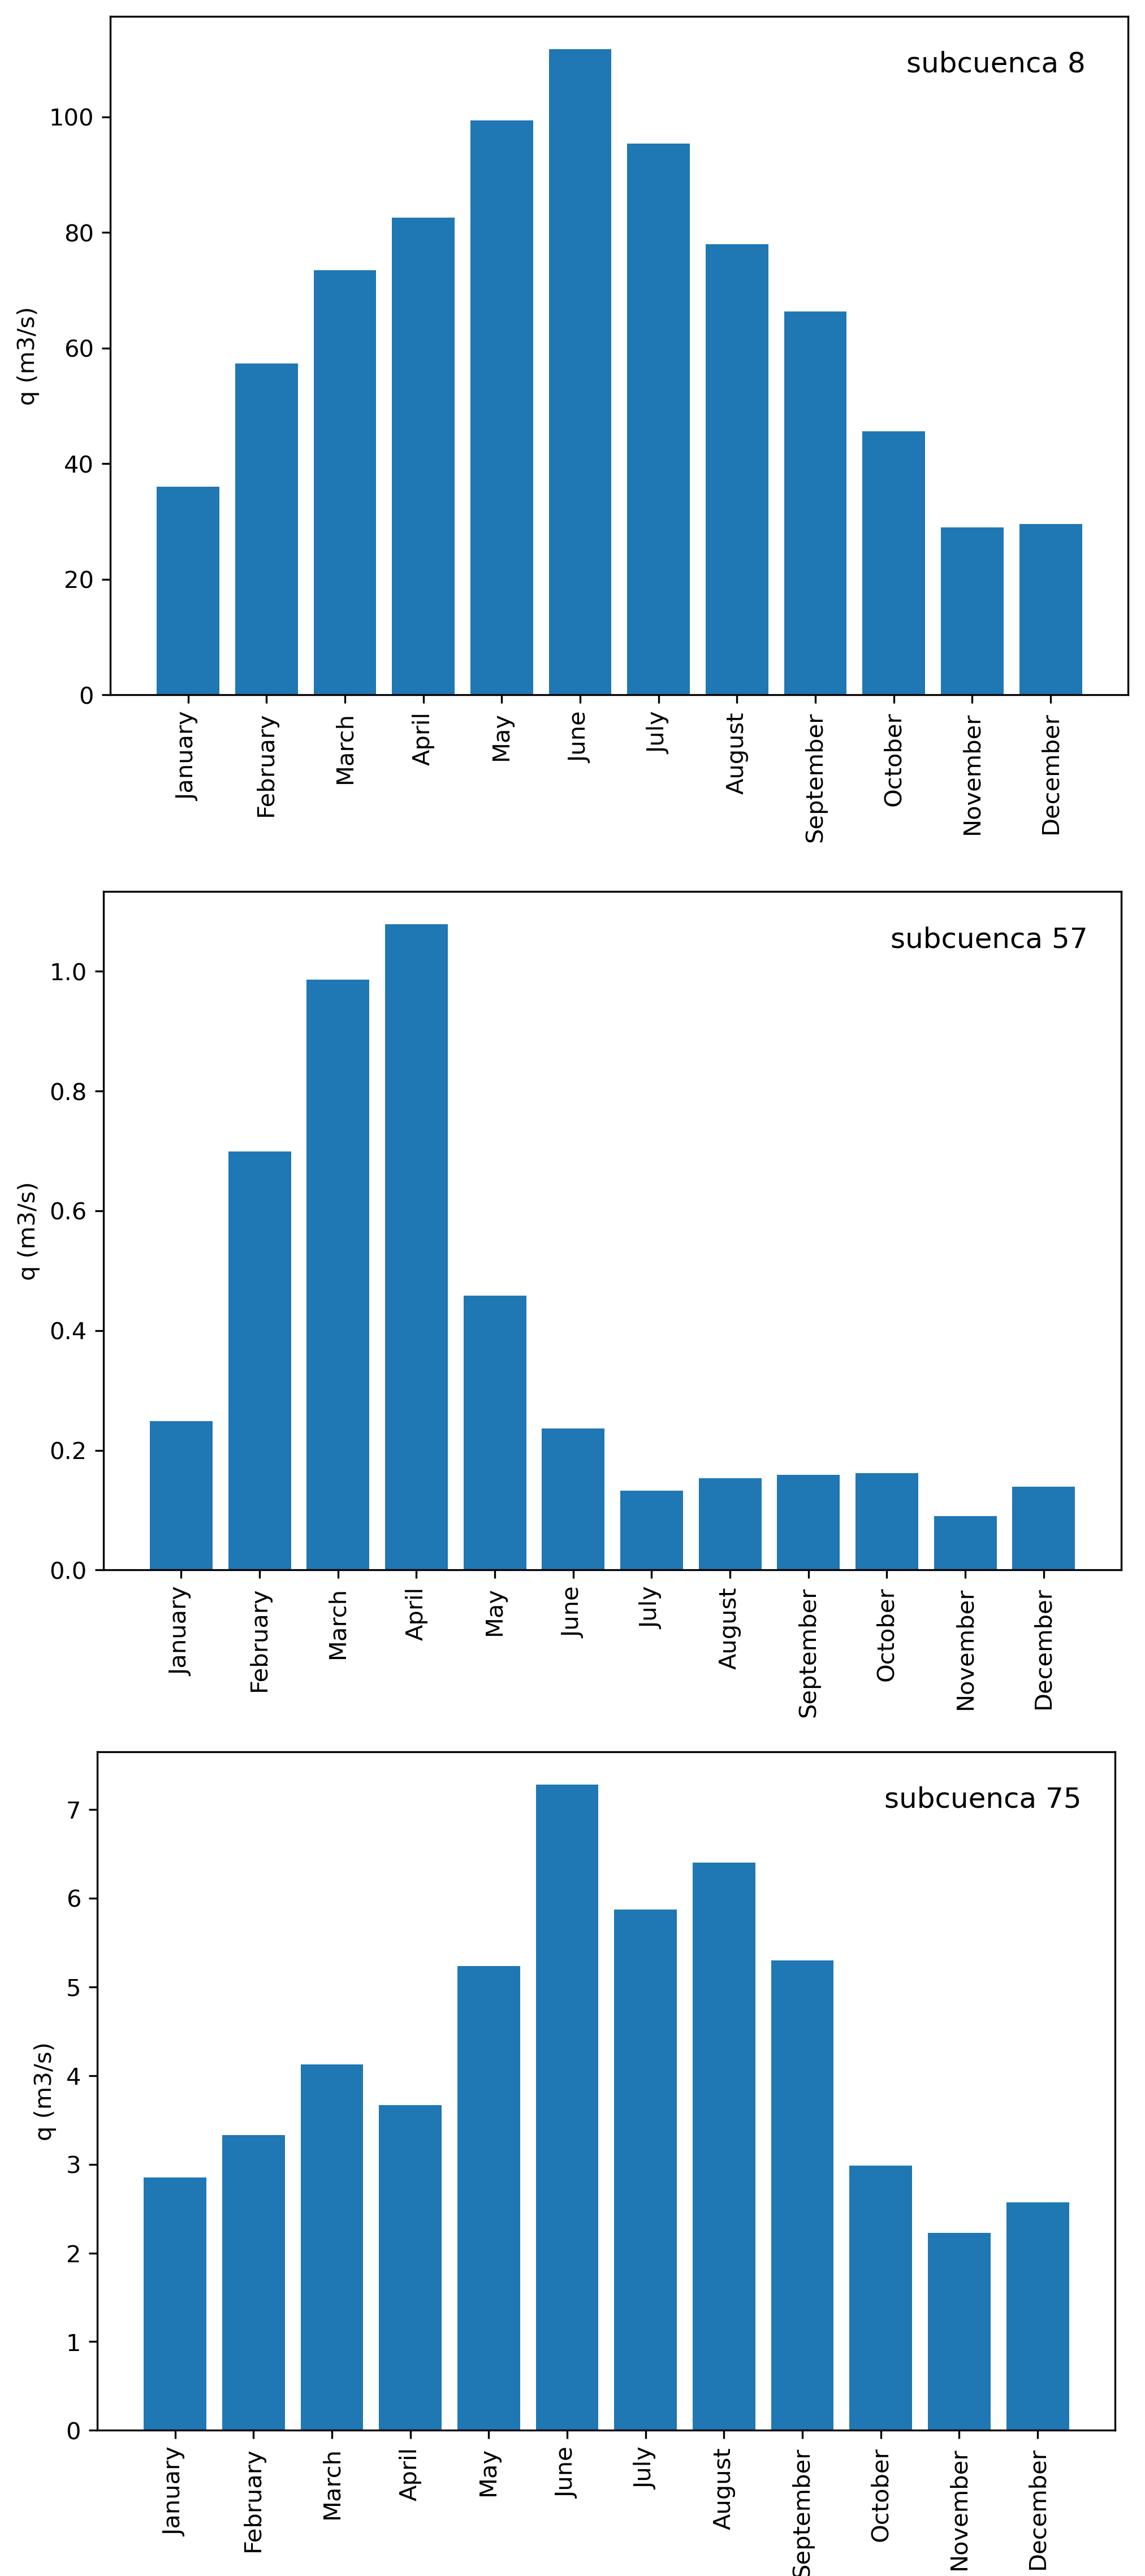
\includegraphics[height=6.5in]{Figures/outputs_MELCA_mensuales.png}
%       \caption{ Valores medios mensuales de caudal natural para tres subcuencas durante los años 2000 y 2020.}
%       \label{6}
%     \end{center}
%   \end{figure}

%  En la figura \ref{5} se muestran graficas con los resultados  para 
% las subcuencas con id 8, 57 y 75 (ver figura \ref{4}). 
% En los paneles superiores se muestras las series de precipitación de entrada y los parámetros del modelo, 
% capacidad de almacenamiento,
% coeficiente de enrutamiento y los factores de corrección. 
% La cuenca más alta es la 75 (?) y posee el mayor factor de corrección fcp,
% la más baja es la 8 y tiene el factor de corrección menor.

% Tal y como vimos en la sección \ref{regimenes_prec}, la subcuenca 8 presenta un regimen de precipitaciones 
% mixto, de las tres cuencas es la que se encuentra más aguas abajo por lo que el caudal medio, ---, es 
% considerablemente superior que en las otras dos. Su area es de --
% la superficie agregada de la cuenca es de --- 
% (sumando la superficie de las cuencas aguas arriba que vierten ella) lo que se produce en una productividad de ---.
% La cuenca 57 se encuentra en la region oeste, presente un regimen bimodal, caudal medio de ---, superficie --- y 
% productividad media de ---, mientras que la cuenca 75 presenta un régimen monomodal y sus valores son---, ---
% y respectivamente.



% En la figura ... se muestran los caudales medios mensuales
% para la salida de la cuenca (subcuenca 73) . El caudal medio es de --- $m^3/s$ 
% este asciende a un valor máximo de ...entre los meses de ... y de ...., y presenta un mínimo de .... entre los meses de ....
% y ..... La superficie agregada de la cuenca es de 3590 $km^2$, con una precipitación media de 1120 $mm$ que se traducen en una 
% productividad de ----.

  

% \subsection{Parámetros físicos}
% \subsubsection{Capacidad máxima de almacenamiento del terreno}

% Las ecuaciones anteriores pueden aplicarse de manera agregada para toda una cuenca, considerada como un ente único, 
% o bien de manera semi-distribuida, considerando varias subcuencas, cada una de ellas con sus parámetros y forzamientos 
% climáticos diferenciados. Si se emplea el modelo en un marco semi-distribuido, es preciso incluir, cuando el paso temporal
%  de cálculo lo requiera, la traslación del flujo desde cada subcuenca al punto de salida. El MELCA es precisamente una 
%  versión semi-distribuida del LEM genérico,
%  con una serie de particularidades que se describen a continuación.

\section{Modelo MODSIM}
\label{Modelo_balance}

Una vez obtenidos los caudales para cada una de las cuencas, ya sea simulados por el modelo LEM o generados por 
los modelos de redes neuronales, se ha determinado el balance hidrológico de la cuenca mediante la utilización 
del software MODSIM \cite{modsim}, mundialmente aceptado y  empleado para simular operaciones en sistemas 
hidrológicos como soporte de decisiones. Este modelo permite incorporar simultáneamente la complejidad física, 
hidrológica y las aspectos institucionales y administrativos del manejo de una cuenca, incluyendo los derechos 
del agua. Además, brinda soporte para la toma de decisión en el uso del agua entre la agricultura, uso poblacional,
 industrial, energético y ambiental.


\begin{figure}[h!]
    \begin{center}
      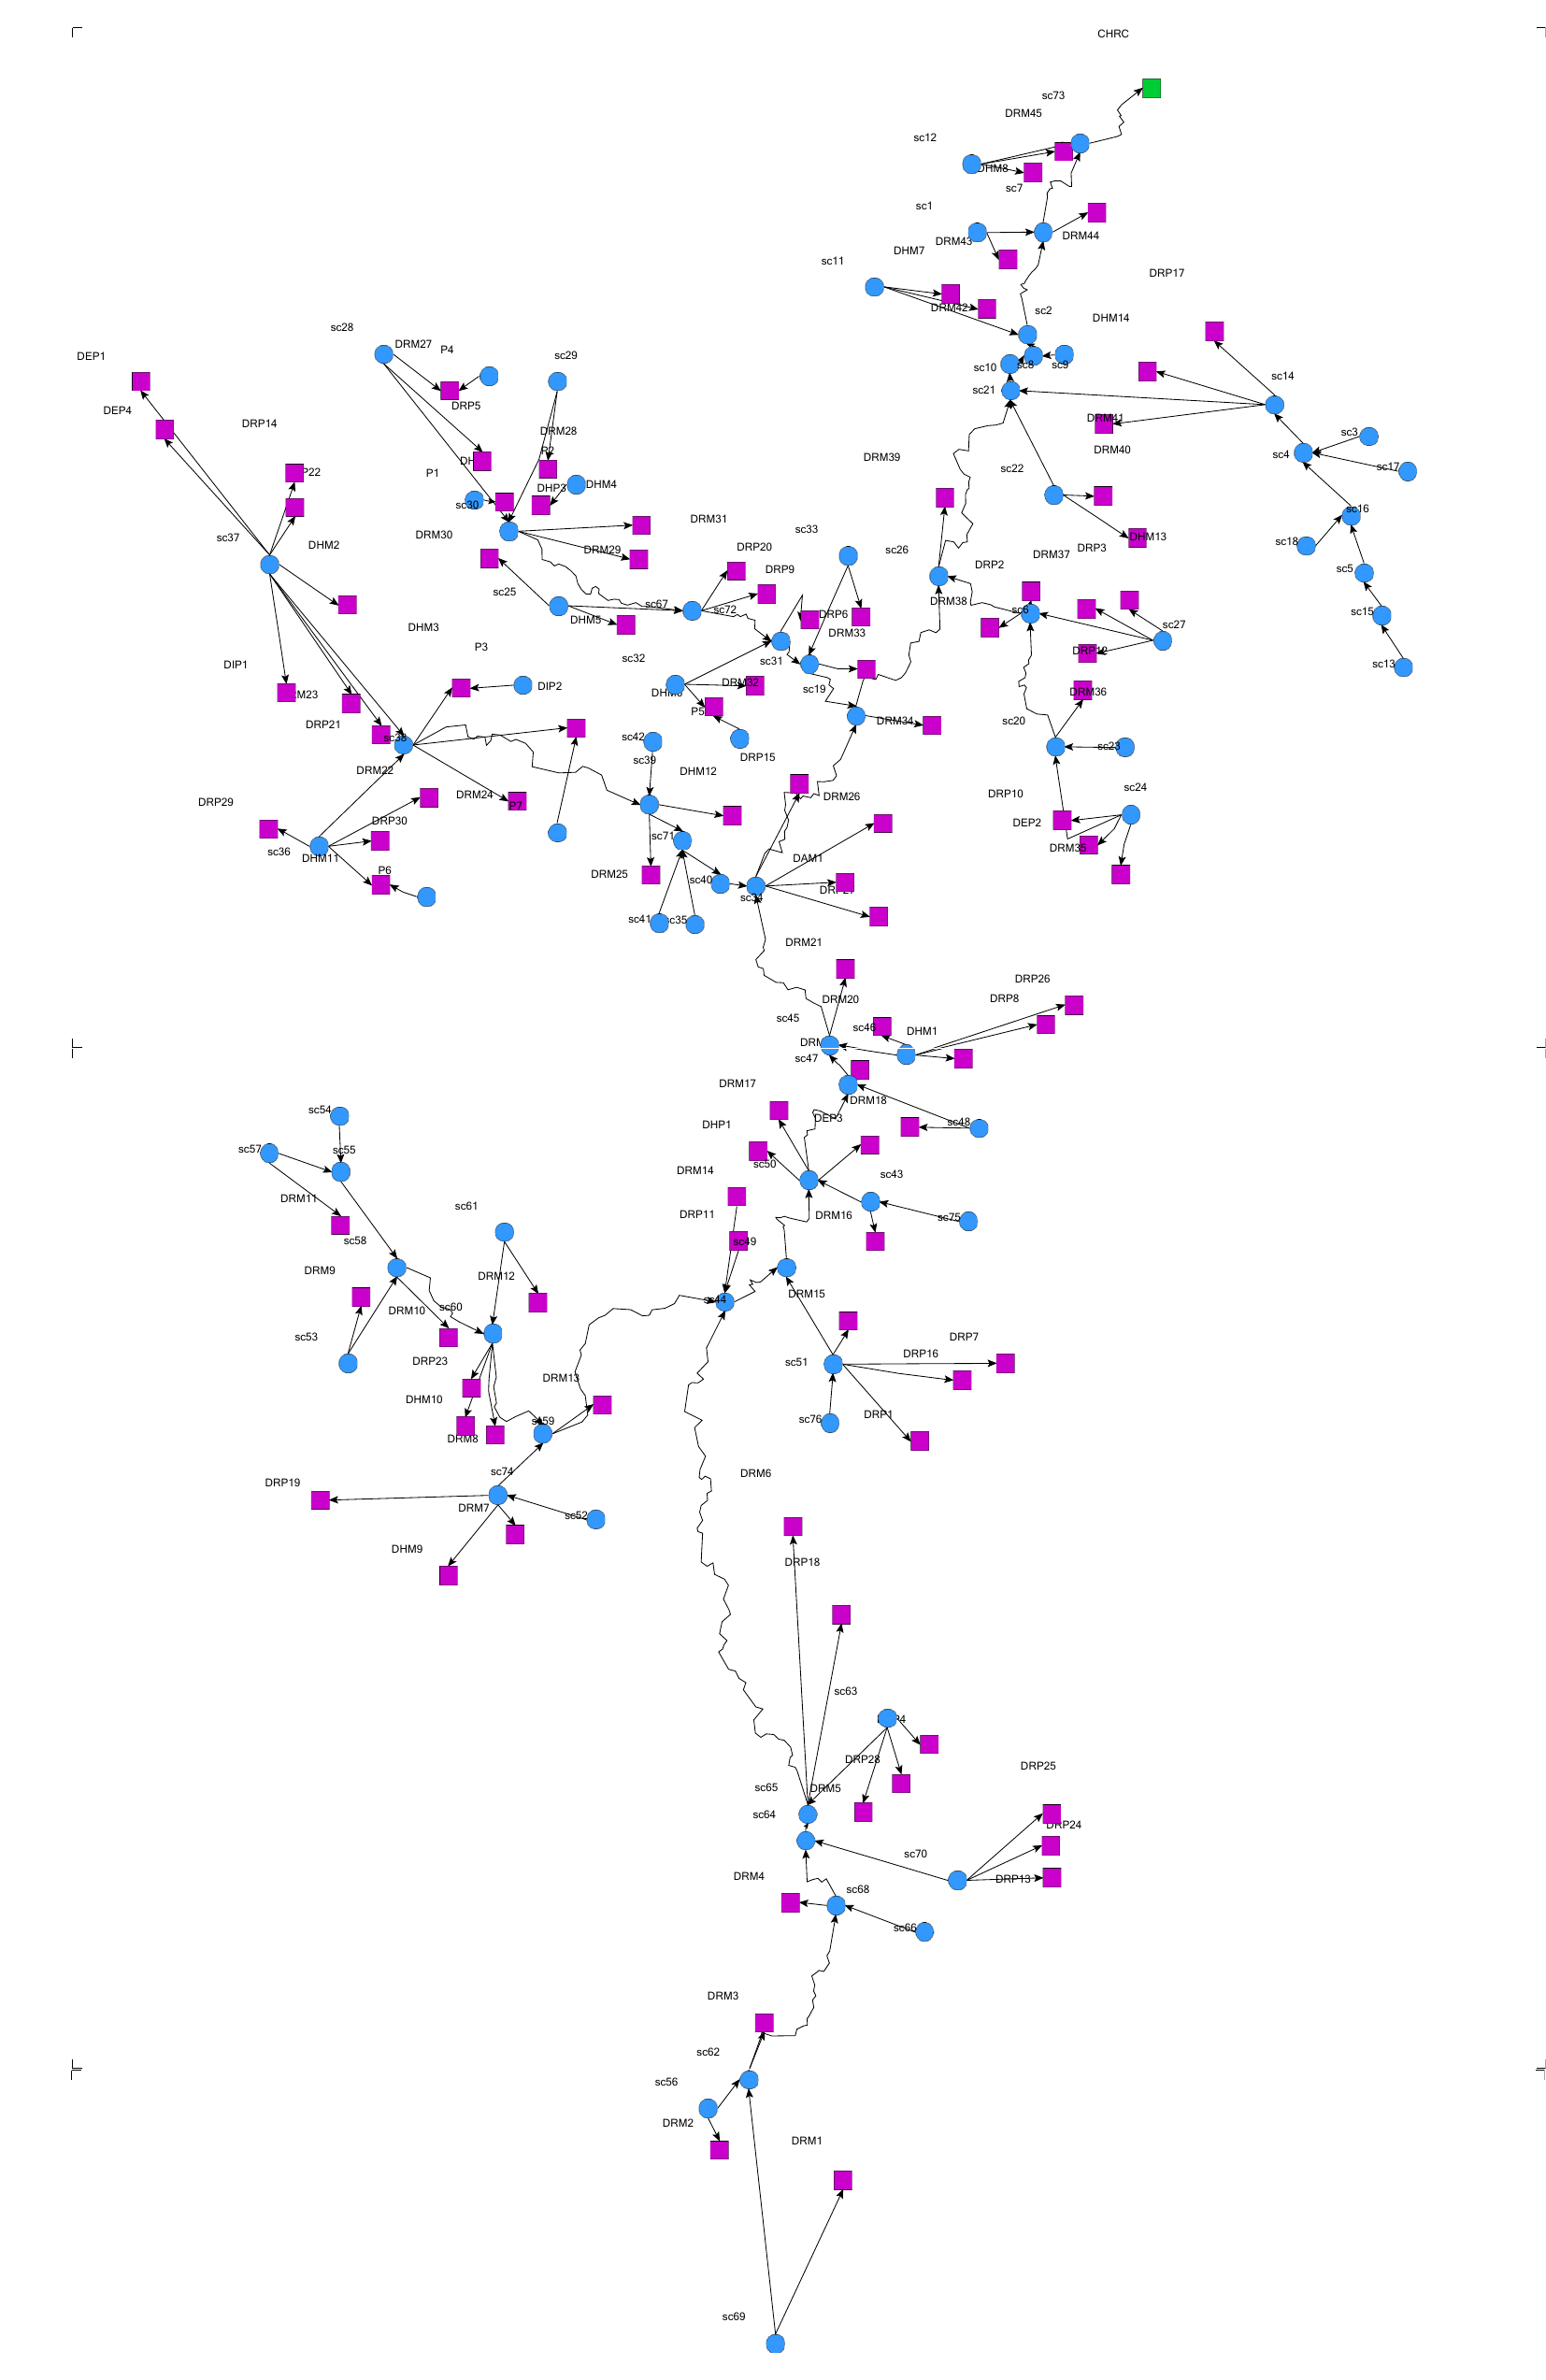
\includegraphics[height=8.5in]{Figures/modzim/figs.png}
      \caption{ Esquema conceptual de CHRC con MODSIM}
      \label{caudales}
    \end{center}
  \end{figure}

  MODSIM es un modelo compuesto por nodos y enlaces que representa el sistema que constituye una cuenca fluvial. 
  Los objetos utilizados en el modelo tienen asociados un costo, representado por un número de prioridad relativo. 
  Los nodos con número de prioridad bajo tendrán menos costo y serán satisfechos antes que los nodos con una prioridad
  mayor. Los objetos en MODSIM no se limitan a representar características físicas e hidrológicas de una cuenca 
  fluvial, sino que también se utilizan para simbolizar elementos artificiales y conceptuales para modelar mecanismos
   administrativos y legales complejos que rigen la asignación de agua. 

   Para optimizar la distribución de agua en las redes del cauce, MODSIM minimiza 
   una función objetivo definida de la siguiente forma \cite{modsim2}:

   \begin{equation}
    \sum_{k \in A}c_k\cdot q_k
   \end{equation}

   donde $q_k$ es el caudal en el enlace $k$, $c_k$ son pesos o las prioridades de derecho de agua por unidad de caudal en
   el enlace $k$. 

   La minimización de esta función debe conservar el balance de masa, es decir, 
   \begin{equation}
    \sum_{k \in O_i} q_k- \sum_{j \in I_i} q_j = b_{it}(q)
   \end{equation}

   \begin{equation}
    l_{kt} < q_k< u_{kt}
   \end{equation}

   donde $O_i$/$I_i$ es el conjunto de todos los enlaces que se originan/terminan en el nodo $i$,  
    y $b_{it}(q)$  es la ganancia o la pérdida en el nodo $i$ en el tiempo $t$. $l_{kt}$ $u_{kt}$ son los
    límites inferior y superior superior especificados, respectivamente, en el flujo en el enlace k en el tiempo t.

MODSIM es capaz tener en cuenta en el cálculo la evaporación, los flujos de retorno de las aguas subterráneas, 
las pérdidas en los canales y los requisitos de flujo en la corriente y resuelve las ecuaciones antes descriptas
con el algoritmo de relajación Lagrangiana RELAX-IV \cite{modim3}.


En la figura \ref{modsim}, se muestra el esquema conceptual que representa a la cuenca CHRC. Los círculos son
nodos sin almacenamiento que representan confluencias y desviaciones de los caudales de la cuenca,
las flechas o links representan los caudales fluyentes entre nodos y los cuadrados las demandas consuntivas de agua.
Se han considerado 4 tipos de demandas diferente: humana con prioridad 1, industrial, riego 
y acuicultura con prioridad 2 y energéticas con prioridad 3.


% Una vez obtenidos los caudales naturales y las demandas en la cuenca del río chambo se pueden calcular los caudales intervenidos
% fluyentes por los tramos de ríos. Para un primer análisis se ha creado un software que calcula para cada una de las subcuencas
% el resultado final de forma agregada teniendo en cuenta los flujos de entrada proveniente de las subcuencas aguas arriba, 
% el flujo del caudal natural local, las demandas de agua en dicha subcuenca y  el caudal de retorno de las demandas que vierten a ese tramo.
% Cabe destacar que para este primer análisis no se han establecido criterios de prioridades de las demandas por lo cual 
% no nos centraremos en un problema de optimización, en cambio consideraremos que todas las demandas tienen las mismas 
% prioridades.

% \begin{equation}
%     q_{total} = q_{entrada}+q_{natural}-q_{demandas}+q_{retornos}
%     \label{caudal_tot}
% \end{equation}

% \begin{figure}[h!]
%     \begin{center}
%       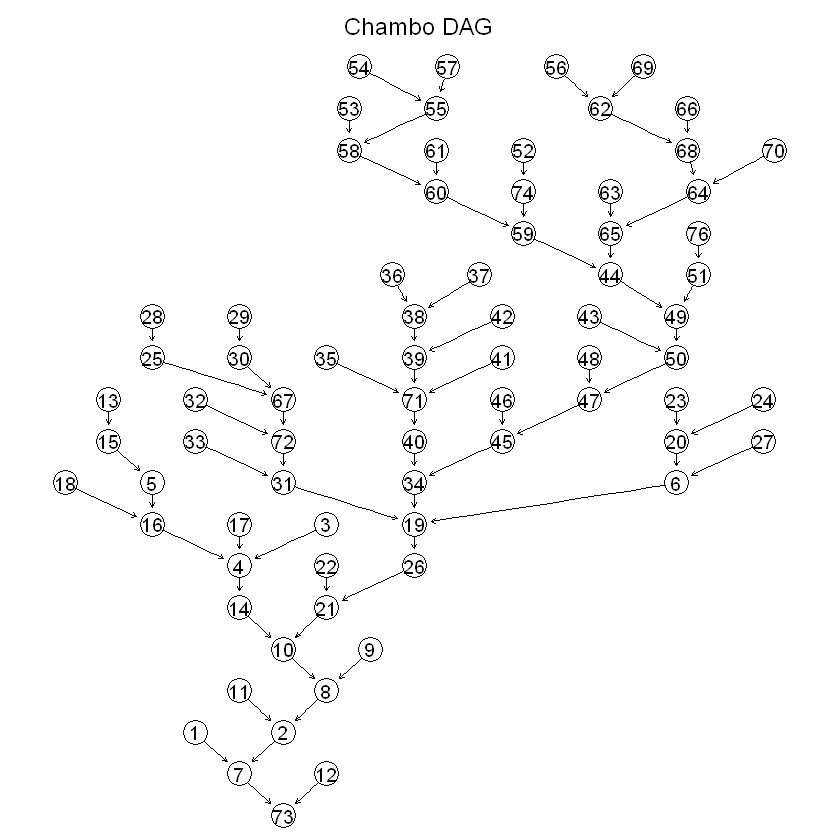
\includegraphics[height=5.in]{Figures/modelo_conceptual_cuenca.png}
%       \caption{Modelo conceptual del entramado de los tramos de la cuenca del río Chambo.}
%       \label{6}
%     \end{center}
%   \end{figure}

% En la figura \ref{6} se muestra una representación conceptual de la cuenca, donde se puede seguir el recorrido de los 
% flujos de aguay la estructura lógica que conecta las diferentes subcuencas y usos de agua. Y en la figura \ref{7} se muestra el 
% diagrama de flujos del programa que calcula el balance hidrológico para cada subcuenca. Este programa realizado en python, 
% realiza las siguientes acciones:

% \begin{enumerate}
%     \item ejecuta el modelo MELCA, cuyo resultado son las series con los caudales para todas las subcuencas de Chambo y selecciona
%     la serie correspondiente al id de la subcuenca de estudio.
%     \item utilizando la matriz de conectividades, cuyas filas  son las cuencas receptoras y cuyas columnas las cuencas 
%     tributarias (ver figura ...) encuentra los ids de las cuencas tributarias.
%     \item encuentra para cada uno de estos ids las demandas totales, seleccionando las filas que satisfacen la condiciones
%     INIC=id (ver tabla demandas) y las agrega. 
%     \item de manera similar calcula los retornos totales, pero esta vez aplicando la condición  FIN=id sobre la tabla demandas 
%     ya que los caudales de retorno son los flujos vertidos aguas abajo por las demandas
%     \item Encuentra las demandas ecosistémicas para cada uno de estos ids y las agrega.
%     \item calcula el resultado final  como en la ecuación \ref{caudal_tot}.
% \end{enumerate}


% A modo de ejemplo, si queremos calcular el caudal resultante para la sub cuenca 68, entonces las cuencas tributarias son las 66 y 62
% (ver figura \ref{6}), estas se obtienen al imponer la condición a la matriz de conectividades, $matcon[66,:]==1$. Una vez se obtienen
% los ids de las cuencas tributarias, se procede a calcular el caudal final como se explica en los puntos 3-6.


% \begin{figure}[h!]
%     \begin{center}
%       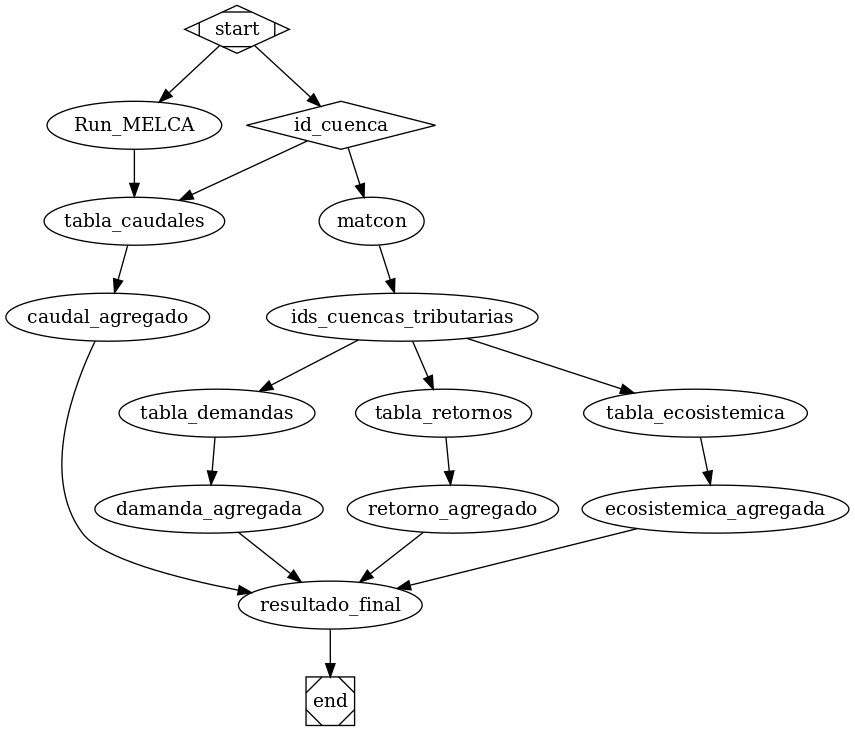
\includegraphics[height=5.in]{Figures/graphviz.png}
%       \caption{Diagrama de flujos del programa que calcula el balance hidrológico de la cuenca.}
%       \label{7}
%     \end{center}
%   \end{figure}

% \section{Modzin}

% Formato de código desde un archivo.

% \vspace{0.7cm}
% \lstinputlisting[style=codigo,language=bash,caption=ejemplo1.sh]{codigo_fuente/ejemplo1.sh}
% \vspace{0.7cm}

% Otro formato de código, para utilizar como salida de ejecución.

% \vspace{0.7cm}
% \begin{lstlisting}[style=terminal,caption=Salida del ejemplo1.sh]
% $ ./ejemplo1.sh 
% 1
% 2
% 3
% 4
% 5
% 6
% 7
% 8
% 9
% 10
% \end{lstlisting}
% \vspace{0.7cm}
\chapter{Resultados}
\label{capitulo 3}
\section{Caudales simulados}

Los resultados finales son obtenidos al aplicar el modelo de balance hídricos, descrito en  \ref{Modelo_balance}, el resultado 
obtenidos es el caudal intervenido, es decir teniendo en cuenta los usos del agua debido a la intervención humana.


\chapter{Análisis de Escenarios}
\label{capitulo 3}
\chapter{Discusiones y Conclusiones}
\label{Discusiones y conclusiones}

Los resultados descritos en el capítulo anterior demuestran que el modelo que realiza los mejores ajustes es el LSTM1 cuando es entrenado en 
el espacio de las componentes principales. Aproximadamente un 70$\%$ de los ajustes obtenidos con el mismo son excelentes mientras que esta cifra  
desciende al 60$\%$ para los modelos denso y LSTM1 entrenado localmente. Si bien los últimos modelos poseen una buena performance en la mayoría de 
las sub-cuencas, presentan mucha variación en el coeficiente de NSE, alcanzando incluso valores negativos en algunos puntos para los cuales 
el modelo LSTM1 PCA arroja resultados que son desde aceptables hasta excelentes. Por otro lado el experimento realizado con el modelo LSTM2, que considera 
un entrenamiento secuencial utilizando solamente los valores de la serie de caudales de descarga de las sub-cuencas, ha demostrado
tener una  mala performance en la mayoría de los puntos. 

Los resultados antes mencionados nos llevan a concluir que la inclusión de las celdas de memoria LSTM y la presencia de componentes principales 
mejoran notablemente la performance de los modelos en cuencas hidrográficas. 
Por un lado las celdas LSTM permiten almacenar información de eje temporal sobre los diferentes procesos  que ocurren en  las sub-cuencas,
y así captar más información sobre la relación entre eventos de precipitación y descarga. Por otro lado, 
las componentes principales reducen considerablemente la dimensión del espacio predictor
y combinan la información proveniente de todo el dominio del mismo, lo que soluciona problemas de sobre ajustes y el problema
des desvanecimiento del loss presente en las cuencas más pequeñas y áridas. 
Finalmente, una vez entrenados lo modelos, se ha demostrado que los resultados obtenidos con redes LSTM
pueden ser utilizados para simular operaciones en la cuenca CHRC, ya que se ha comprobado que
el resultado del balance hidrológico obtenido con MODSIM es el mismo que los obtenidos con los valores simulados por el modelo LEM.

Todos estos resultados apuntan en la misma línea que estudios recientes en los cuales se concluye que 
las redes neuronales generalmente requieren una gran cantidad de datos de entrenamiento y que 
los ajustes que se obtienen al entrenar modelos de aprendizaje profundo en una sola sub-cuenca no suelen ser fiables \cite{Kratzert}. 
Esto supone una gran diferencia con el modelado y calibrado hidrológico tradicional que normalmente demuestra una mejor performance 
cuando los modelos se calibran de forma independiente para cada sub-cuenca.
Ésta propiedad de los modelos clásicos presenta problemas, ya que se ha observado que los 
 parámetros obtenidos por extrapolaciones  basadas en valores calibrados en cuencas de referencia 
pueden dar lugar a espacios de parámetros poco realistas\cite{Mizukami}. 
Los modelos LSTM en cambio, demuestran tener la capacidad de aprender simultáneamente relaciones de series temporales 
y espaciales en el mismo marco predictivo, lo que evita muchos problemas que actualmente se encuentran 
asociados con la estimación y transferencia de parámetros de modelos hidrológicos tradicionales \cite{Kratzert}, \cite{nearing}.

Una conclusión importante es entonces que las celdas LSTM son capaces de generar un modelo único a partir de grandes conjuntos de datos  
capaz de reflejar los comportamientos hidrológicos regionales específicos de cada sub-cuenca
ya que estos modelos  vinculan las características locales de las sub-cuencas y aprenden
un modelo general a partir de los datos combinados de todas ellas. 
Es por esto que concluimos que la principal virtud de las redes neuronales no es simplemente el hecho de que ajusten bien sino su capacidad de
aprendizaje y  flexibilidad para ser utilizadas en una variedad de  lugares y condiciones diferentes.


Por último, como posibles mejoras para trabajos futuros se propone concatenar los descriptores estáticos de las sub-cuencas, 
como por ejemplo el área, la longitud del cauce, etc., al espacio predictor. Otra mejora podría ser definir una función objetivo al 
entrenar los modelos que no dependa del valor medio de los caudales de descarga de las diferentes cuencas. Kratzert etal. \cite{Kratzert} 
proponen por ejemplo usar directamente una definición global del coeficiente de Nash-Stutcliffe durante el entrenamiento
de los datos. En este caso, si bien se perdería la linelidad entre las métricas del RMSE y el NSE,  esto permitiría 
contemplar el hecho de que las variancias de los datos observacionales difieren en distintas cuencas y así evitar el sobre-peso 
asociado a las cuencas más grandes y húmedas.


\bibliographystyle{babunsrt}
\bibliography{bibliografia}

\end{document}